\documentclass[a4paper,12pt]{article}
\usepackage{amsmath}
\usepackage{graphicx}
\graphicspath{ {images/} }
\usepackage[utf8]{inputenc}
\usepackage[english]{babel}
\usepackage[document]{ragged2e}
 
\begin{document}\begin{flushleft}\newline \textbf{6.819 PSET 2}
\newline \textbf{09/22/2017}
\end{flushleft}
\newline \begin{center}\textbf{ISAAC KONTOMAH}
\end{center}
\begin{flushleft}
\newline \emph{Collaborators:Abdurrahman Akkas,Devin Morgan , Suman Nepal ,Sanchit Bhatta }
\end{flushleft}

\newline \textbf{1.} \emph{\textbf{Hybrid Images}}
\begin{document}
\newline I use a gaussian blur , with gaussian kernel and gaussian parameter $12$
 
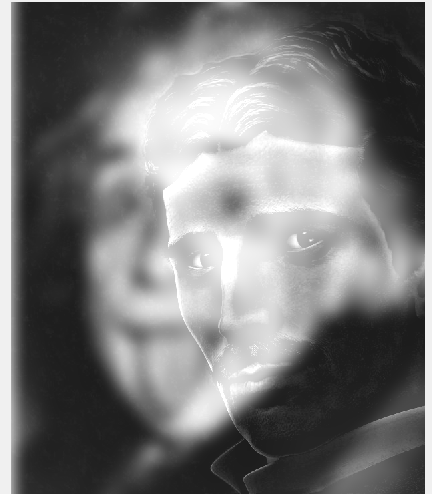
\includegraphics[width = 4cm height = 4cm]{ein_tes.jpg}
 
Image of Einstein and Tesla

 \newline \textbf{2.} \emph{\textbf{De-Hybridizing}}
 \begin{document}
\newline Low frequeny Image
 
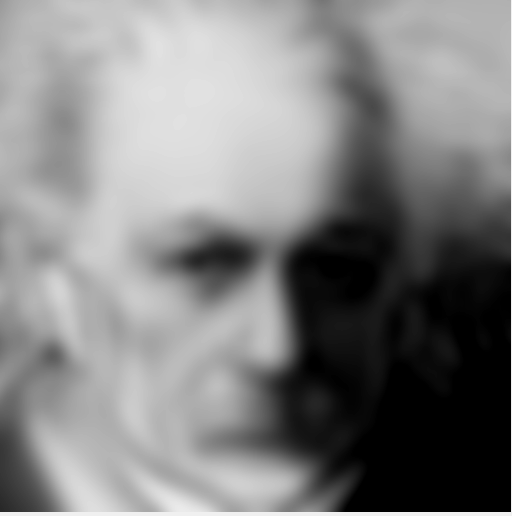
\includegraphics{low_freq_blur.jpg}
 
\newline Dehybridized low frequency image

\begin{document}
\newline Low frequeny Image
 
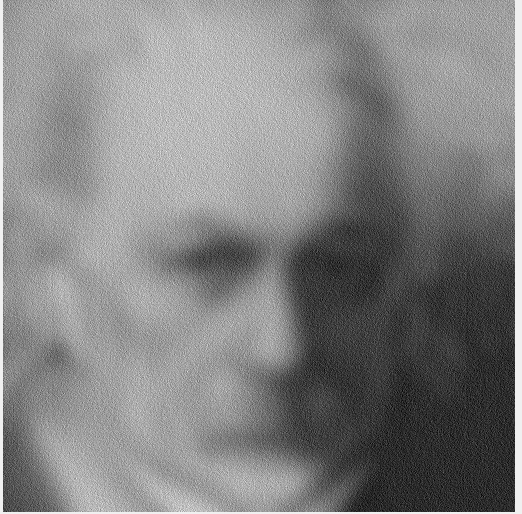
\includegraphics{low_freq_deblur.jpg}
 
\newline Dehybridized low frequency image
 \begin{document}
\newline High frequeny Image
 
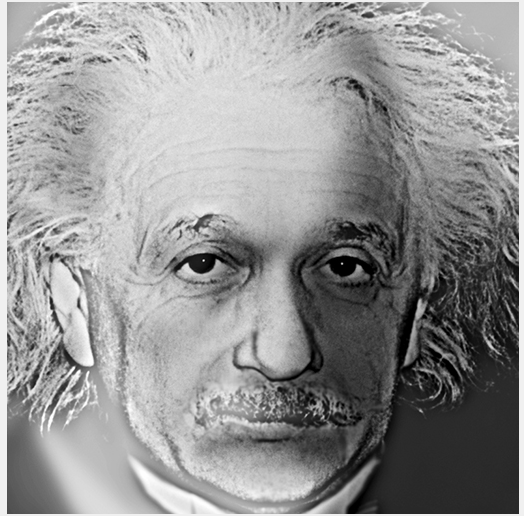
\includegraphics{better_einstein.jpg}
 
\newline Dehybridized high frequency image
 
\newline \textbf{3.} \emph{\textbf{Depth Based Focusing}}

 \begin{document}
\newline Gaussian filtering of image 
 
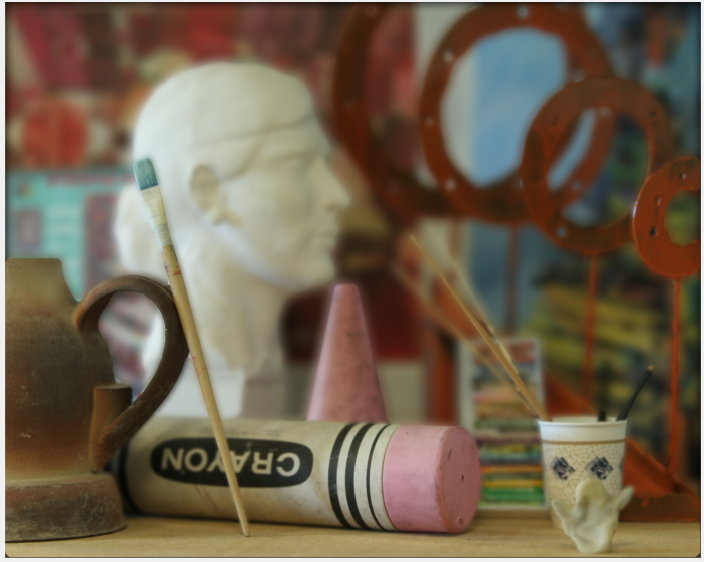
\includegraphics{gauss_filt.jpg}
 
Gaussian filtering done on image
 \begin{document}
\newline Binomial filtering of image 
 
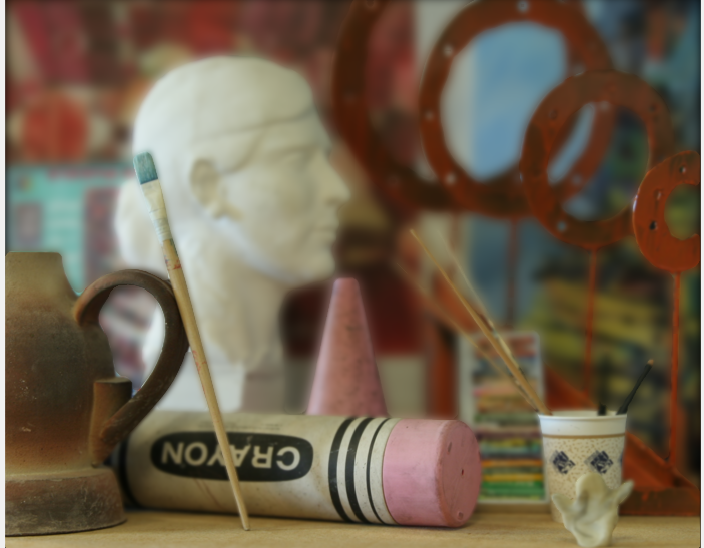
\includegraphics{Bin_filt.jpg}
 
Binomial filtering done on image


\end{document}